% July 2015
% Autor: Mandy Vogel
% Tests 
\documentclass[xcolor={table}]{beamer}
\usetheme{Singapore}

%% \usepackage{listings}
\usepackage{linkimage}

\begin{document}

\title{Recap Location Tests}   
\author{Mandy Vogel} 
\date{\today}
%\logo{\includegraphics[scale=0.14]{PIC1}}

\begin{frame}
\titlepage
\end{frame}

\begin{frame}
\frametitle{Table of Contents}\tableofcontents
\end{frame}

\section{ggplot2}
\subsection{Bivariate Data}
\begin{frame}[fragile,allowframebreaks]\frametitle{Scatter plots}
  \begin{itemize}
  \item up to now we only visualized univariate numerical data but we already used a central geom for visualizing bivariate data 
  \item to produce a scatter plot we use \texttt{geom\_point()} with the aesthetics \texttt{aes(x = variable1, y = variable2)}
  \item we can customize the size (\texttt{size}), shape (\texttt{shape}), colour(\texttt{colour} and \texttt{fill}), and transparency (\texttt{alpha}) of the points 
  \begin{center}
    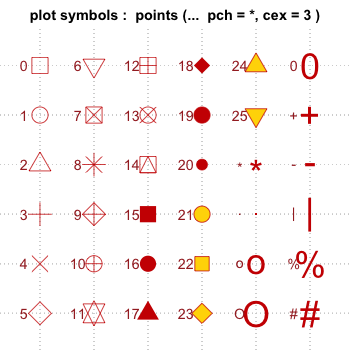
\includegraphics[width=6cm]{shapes.png}
  \end{center}
  \end{itemize}
\end{frame}

\begin{frame}[fragile]\frametitle{Scatter plots}
\small
\begin{verbatim}
> ggplot(GaltonFamilies, aes(x=mother,y=father)) +
+     geom_point()
\end{verbatim}
which results in:
\end{frame}


\begin{frame}\frametitle{Scatter plots}
  \begin{center}
    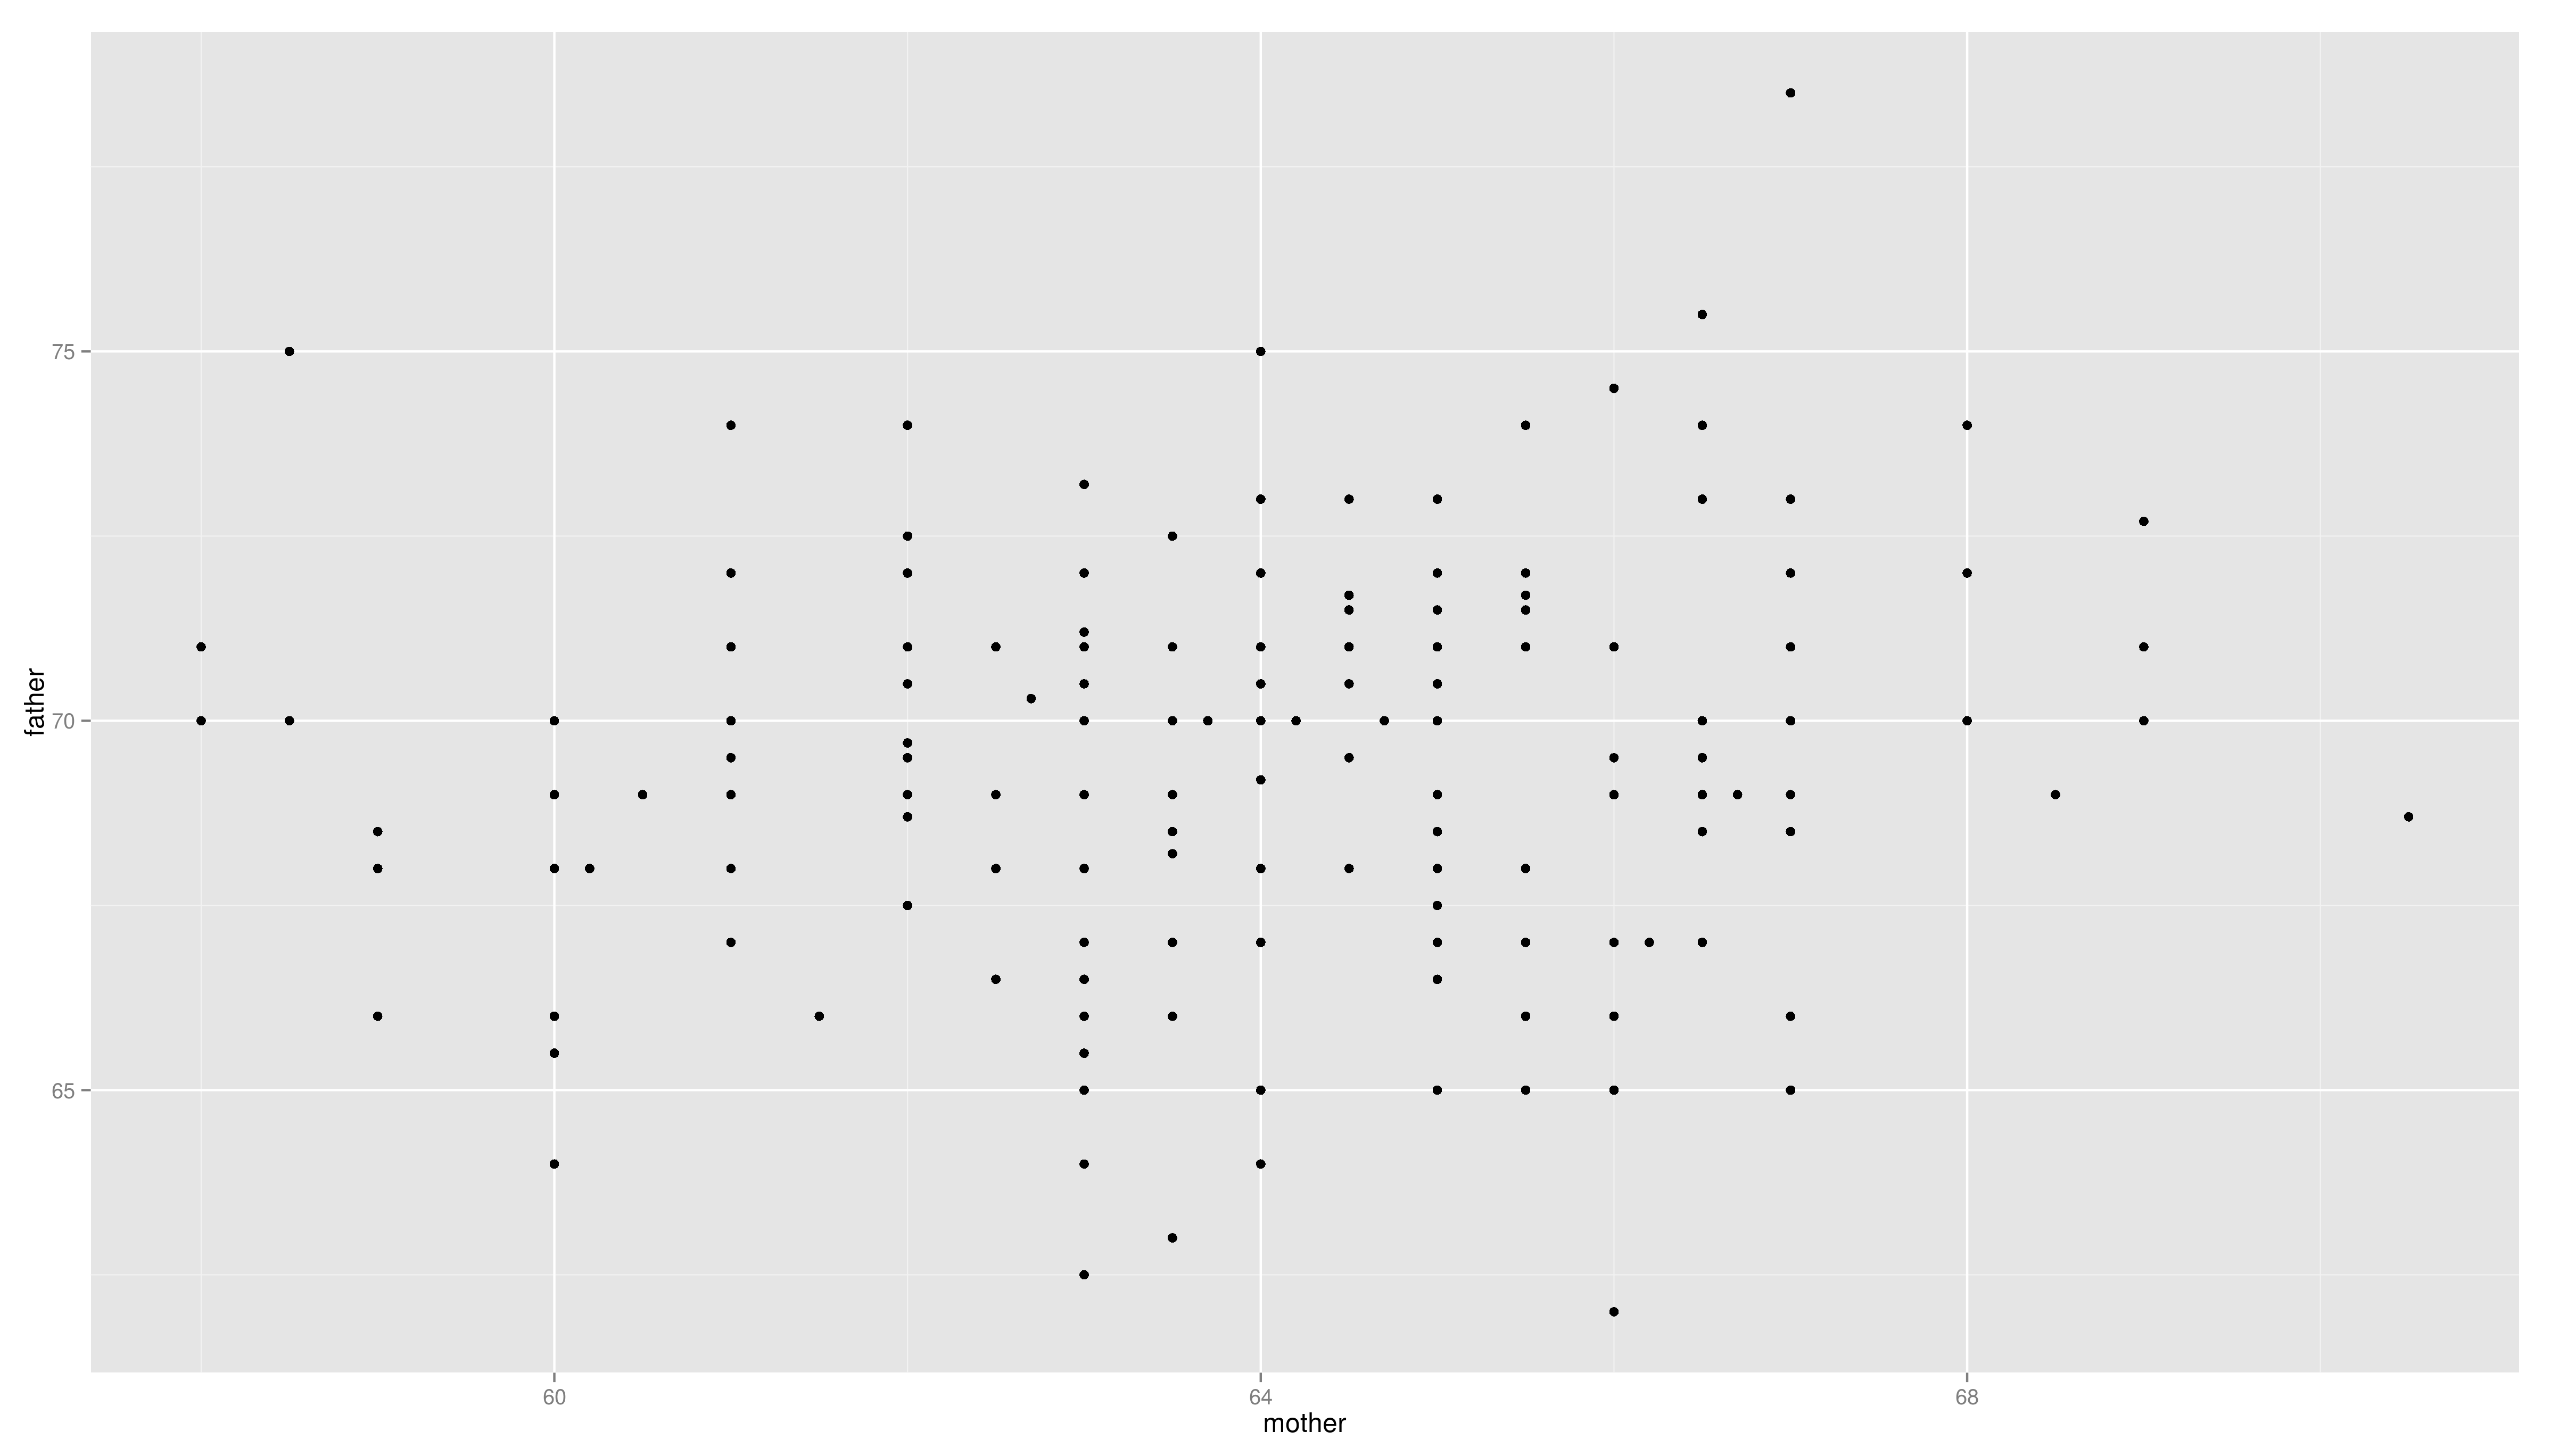
\includegraphics[width=9cm]{scatter.png}
  \end{center}
\end{frame}

\begin{frame}[fragile]\frametitle{Adding trend lines}
  \begin{itemize}
  \item a trend line is a statistical summary of a bivariate relationship
  \item there are many different trend lines that can be added to a scatterplot
  \item they are easily added through \texttt{geom\_smooth()}
  \end{itemize}\small
\begin{verbatim}
> ggplot(GaltonFamilies, aes(x=mother,y=father)) +
+     geom_point()
\end{verbatim}
which results in:
\end{frame}


\begin{frame}\frametitle{Adding trend lines}
  \begin{center}
    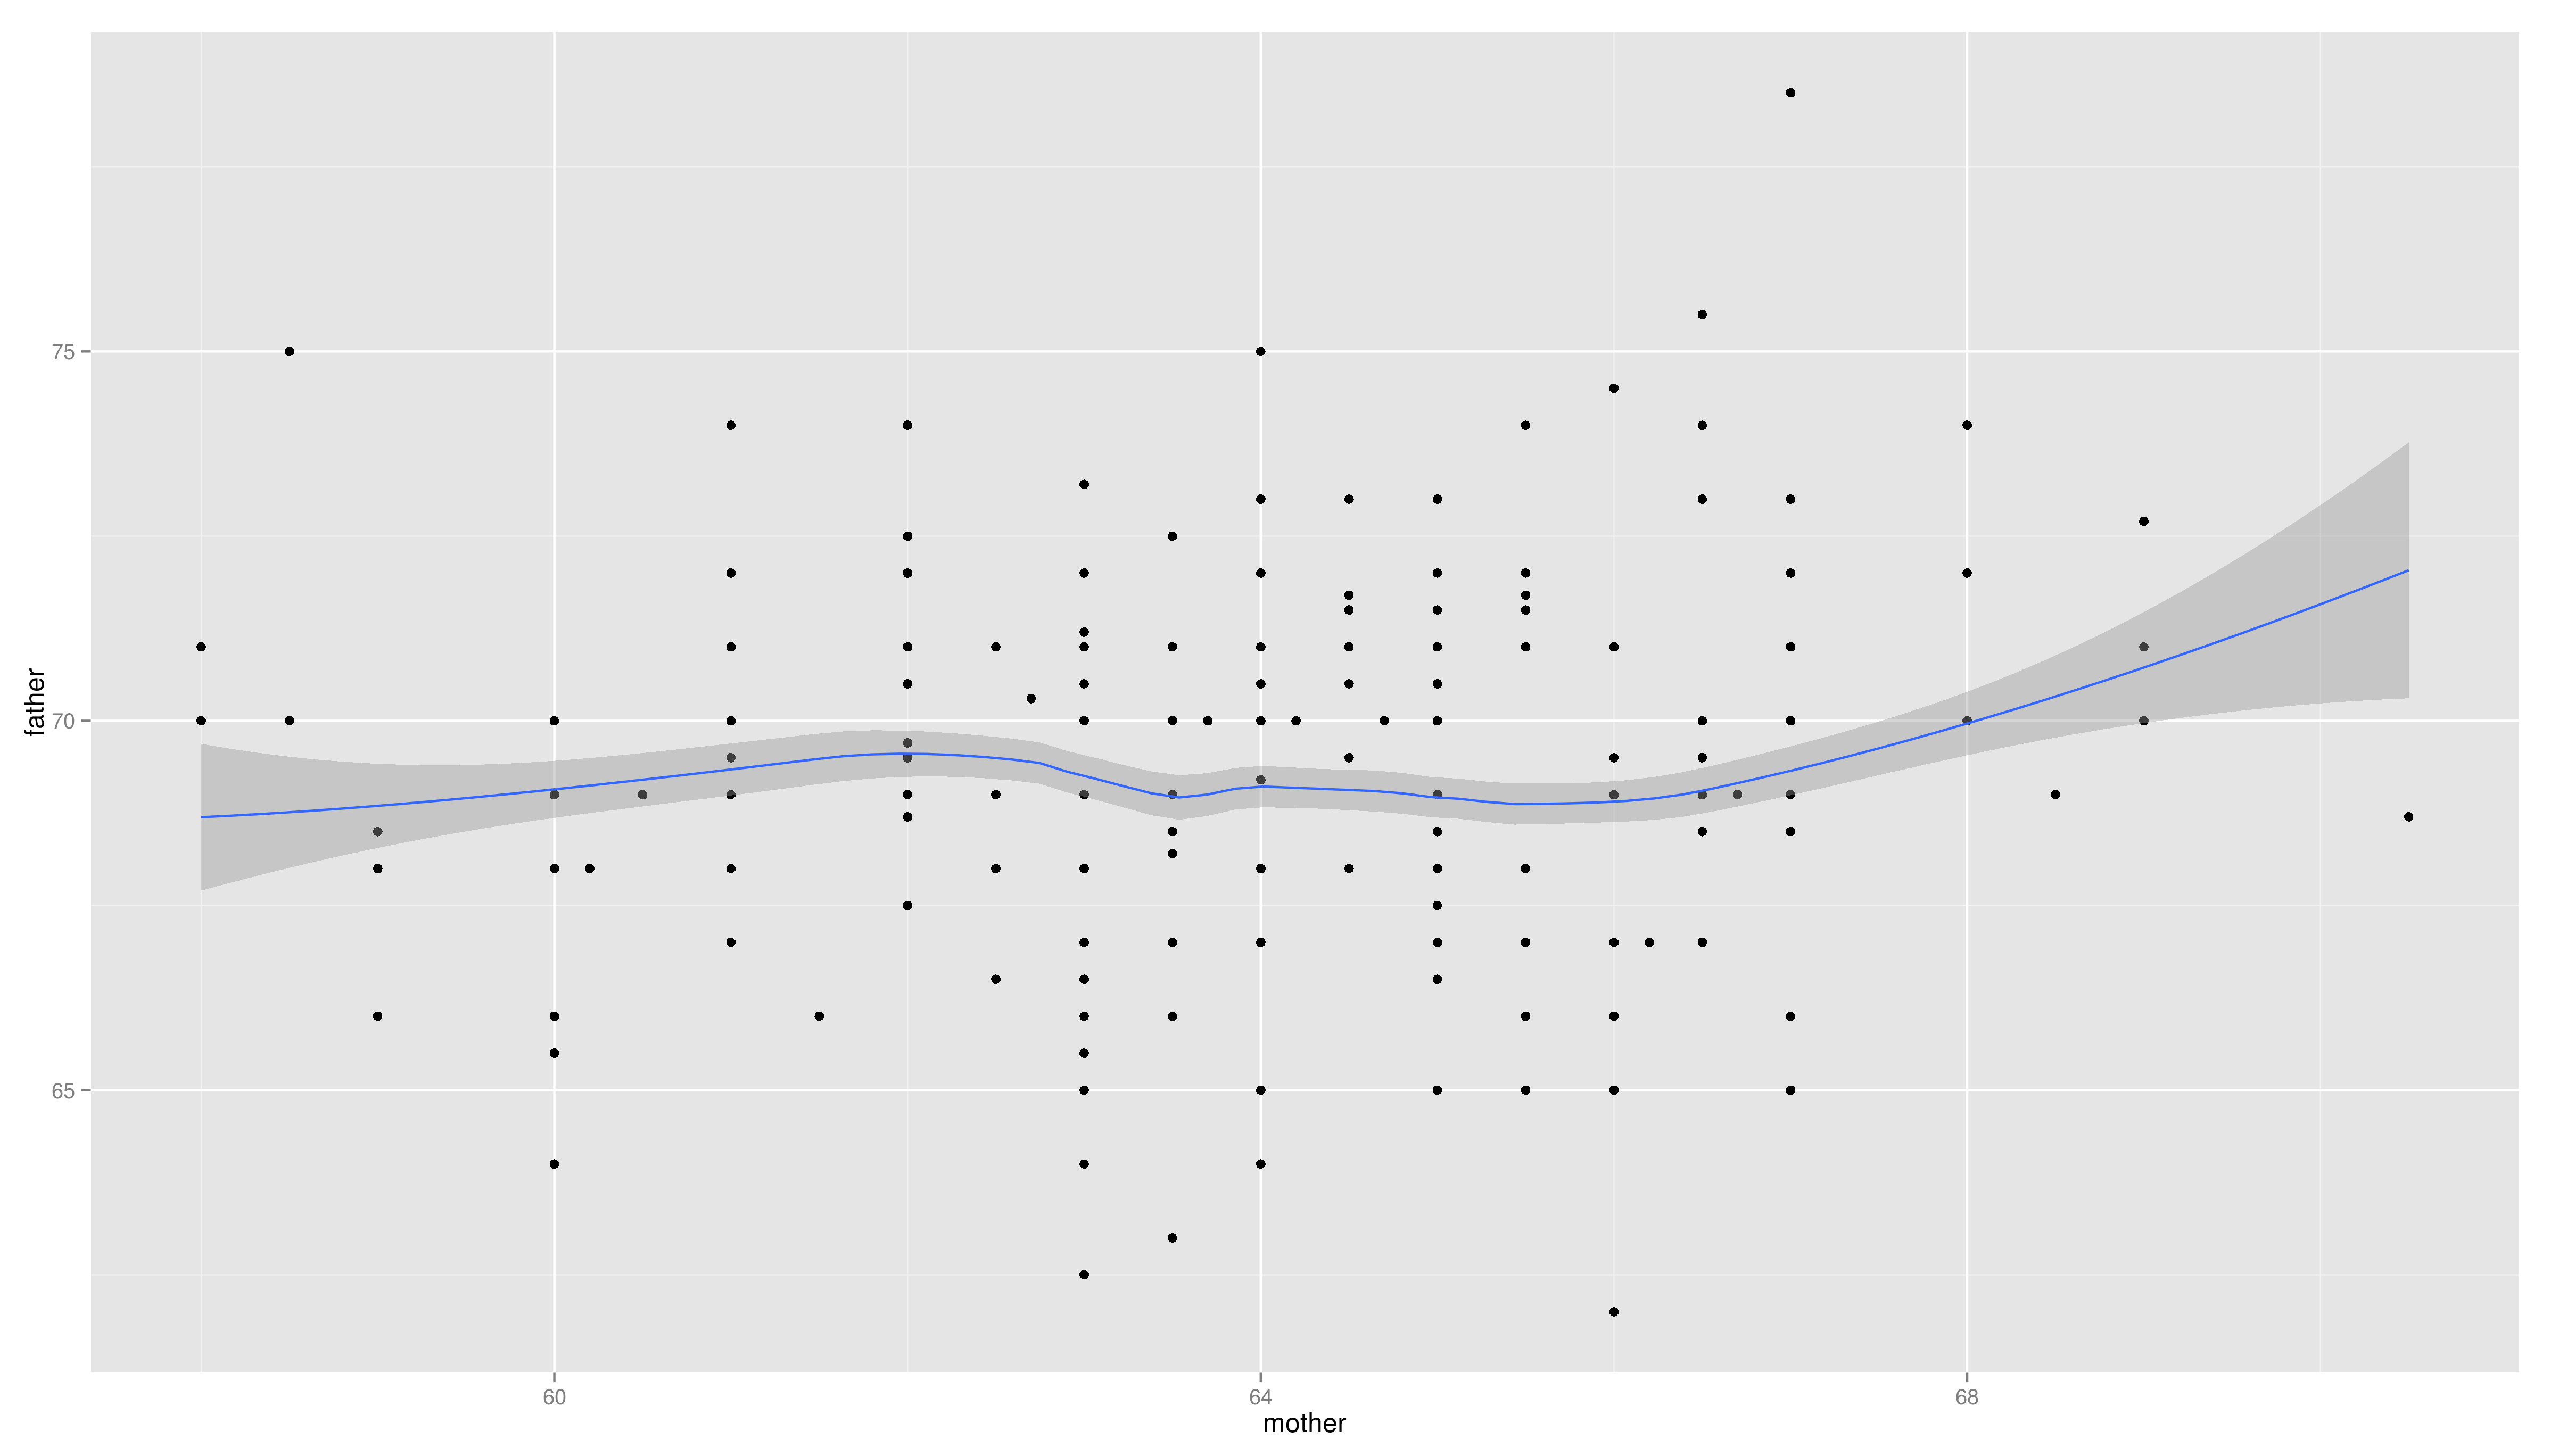
\includegraphics[width=9cm]{scattertrend1.png}
  \end{center}
\end{frame}


\begin{frame}[fragile]\frametitle{Adding trend lines}
  \begin{itemize}
  \item by default \texttt{geom\_smooth()} produces a non-parametric trend line (local polynomial regression fitting for n<1000 otherwise generalized additive model)
  \item we can set a model using the \texttt{method} argument
  \end{itemize}\small
\begin{verbatim}
> ggplot(GaltonFamilies, aes(x=mother,y=father)) +
+     geom_point()
\end{verbatim}
which results in:
\end{frame}


\begin{frame}\frametitle{Adding trend lines}
  \begin{center}
    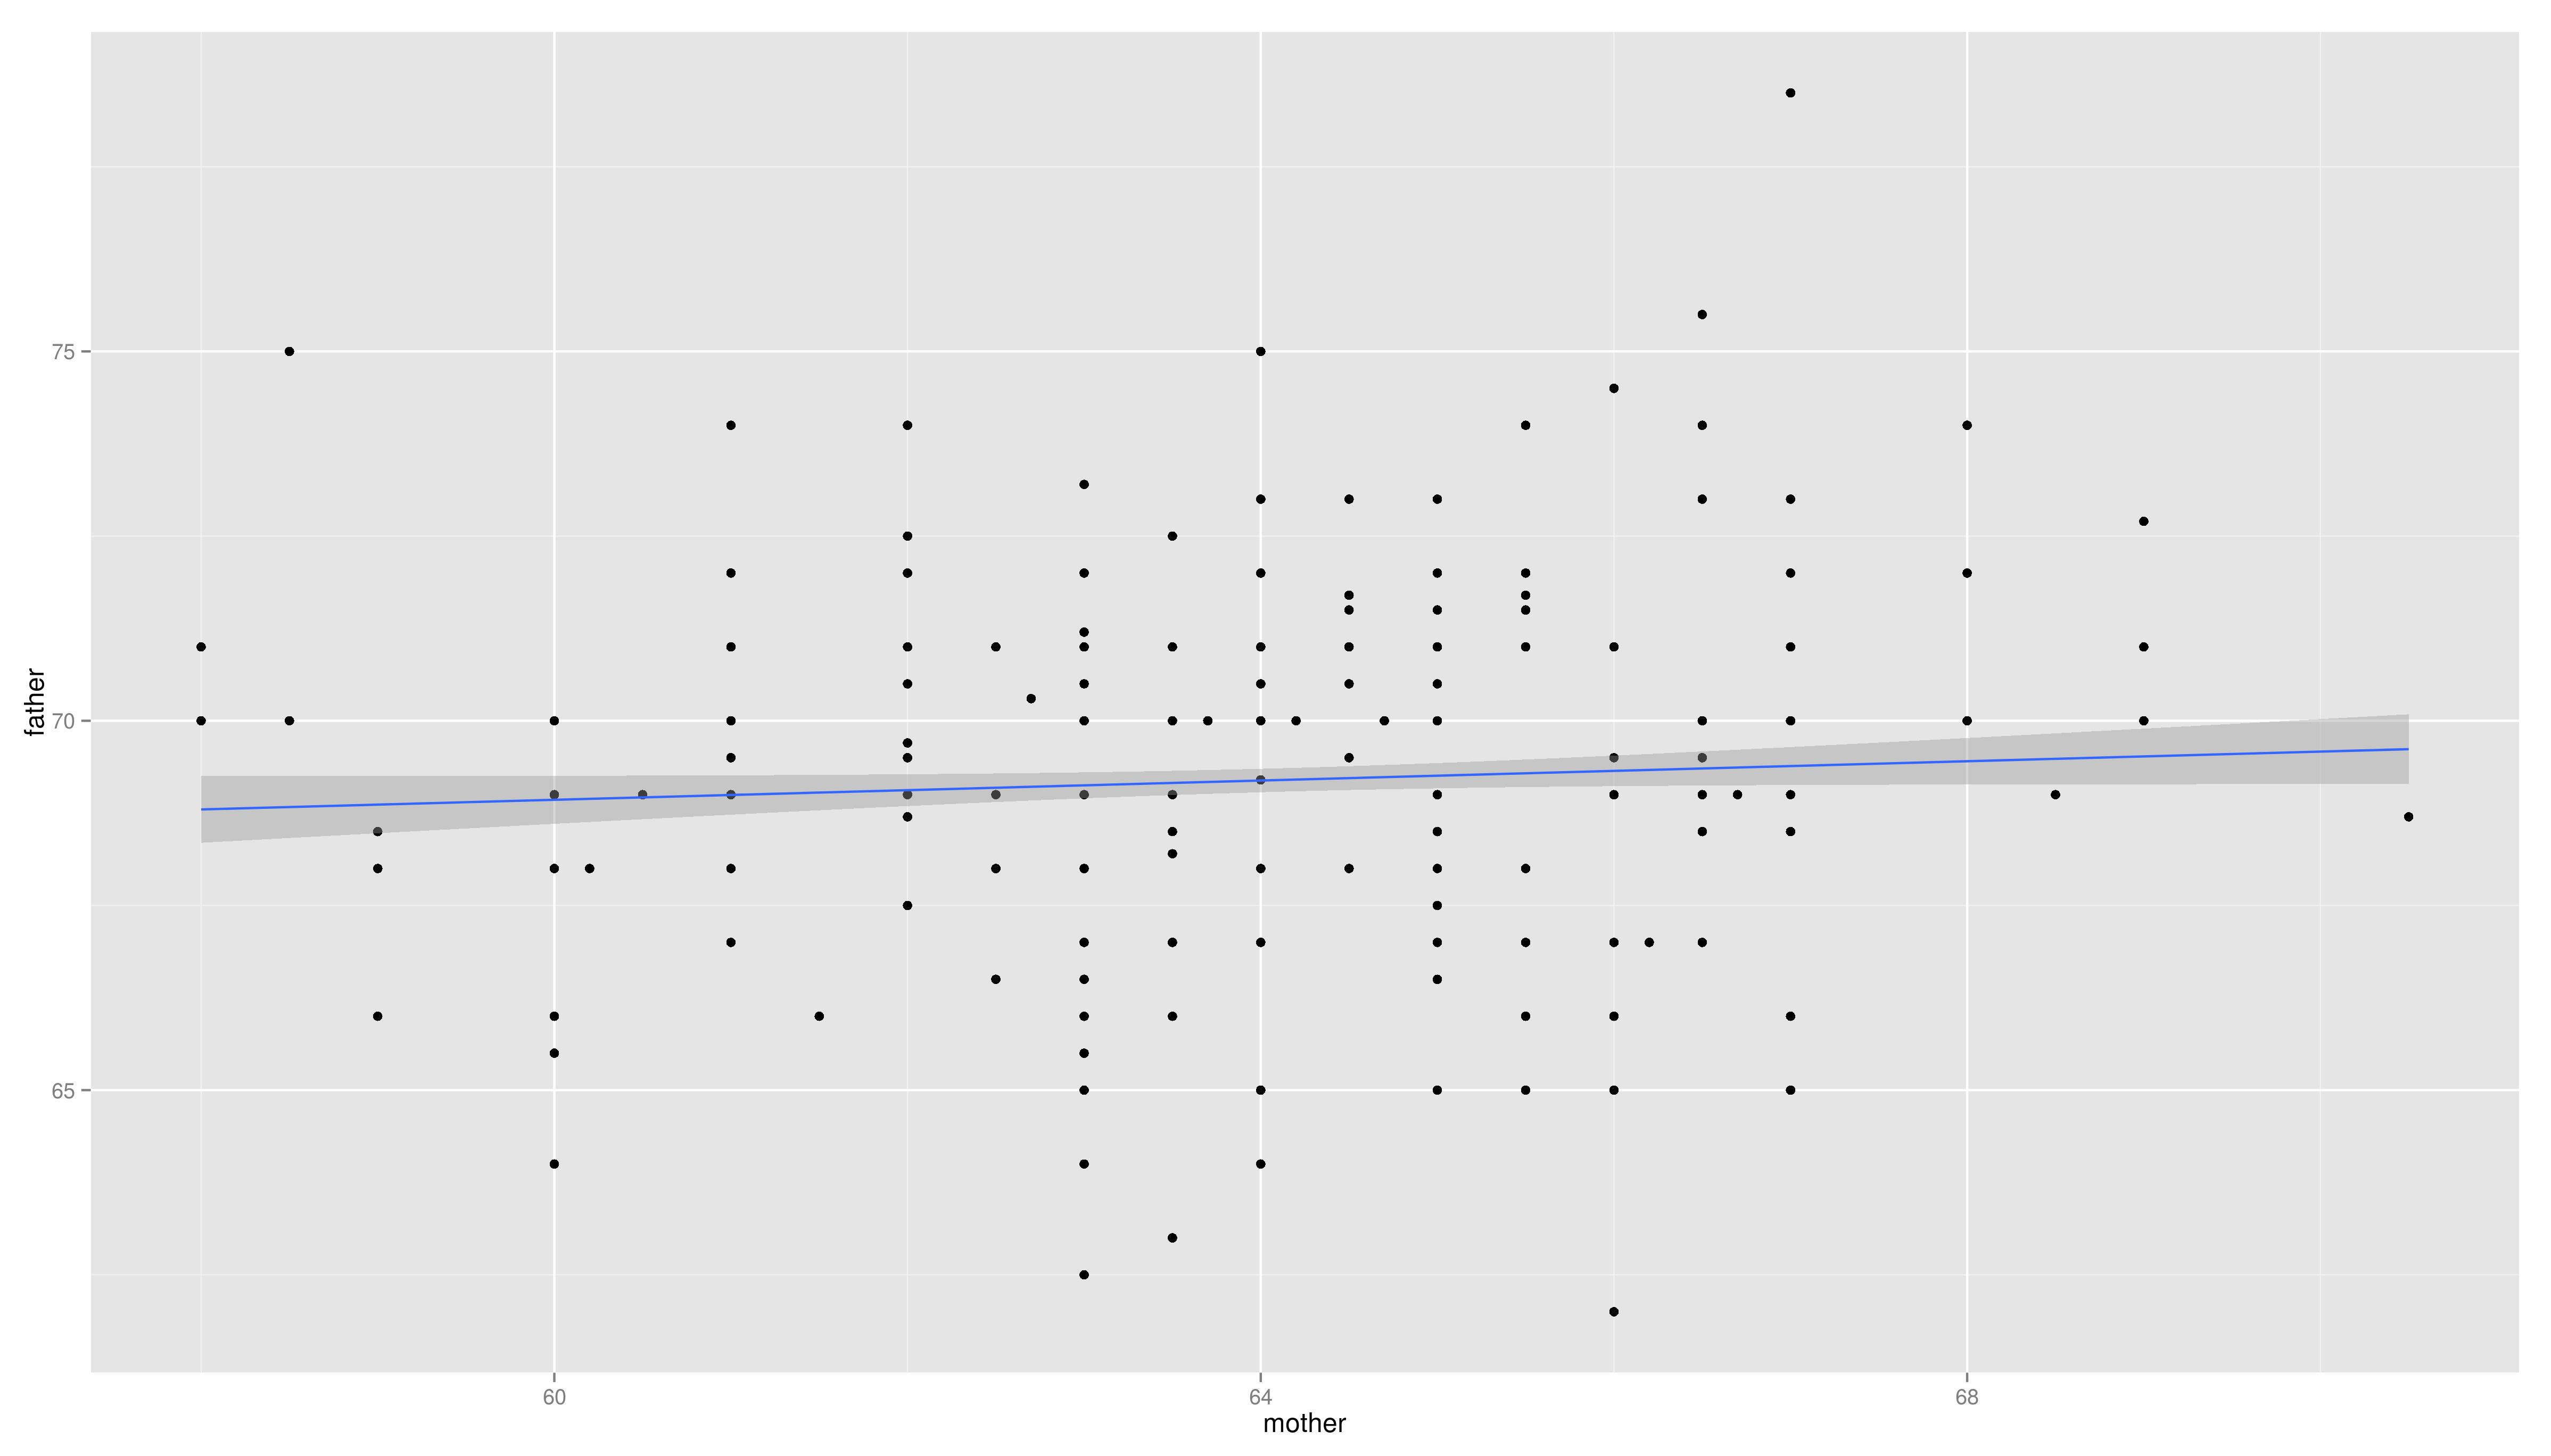
\includegraphics[width=9cm]{scattertrend2.png}
  \end{center}
\end{frame}


\begin{frame}[fragile]\frametitle{geom\_dotplot()}
  \begin{itemize}
  \item it sounds a bit like point, but the function is totally different
  \item infact it is a alternative for histograms for small sample sizes
  \end{itemize}\small
\begin{verbatim}
> ggplot(mtcars, aes(x = mpg)) + geom_dotplot()
\end{verbatim}
which results in:
\end{frame}

\begin{frame}\frametitle{dot plot example}
  \begin{center}
    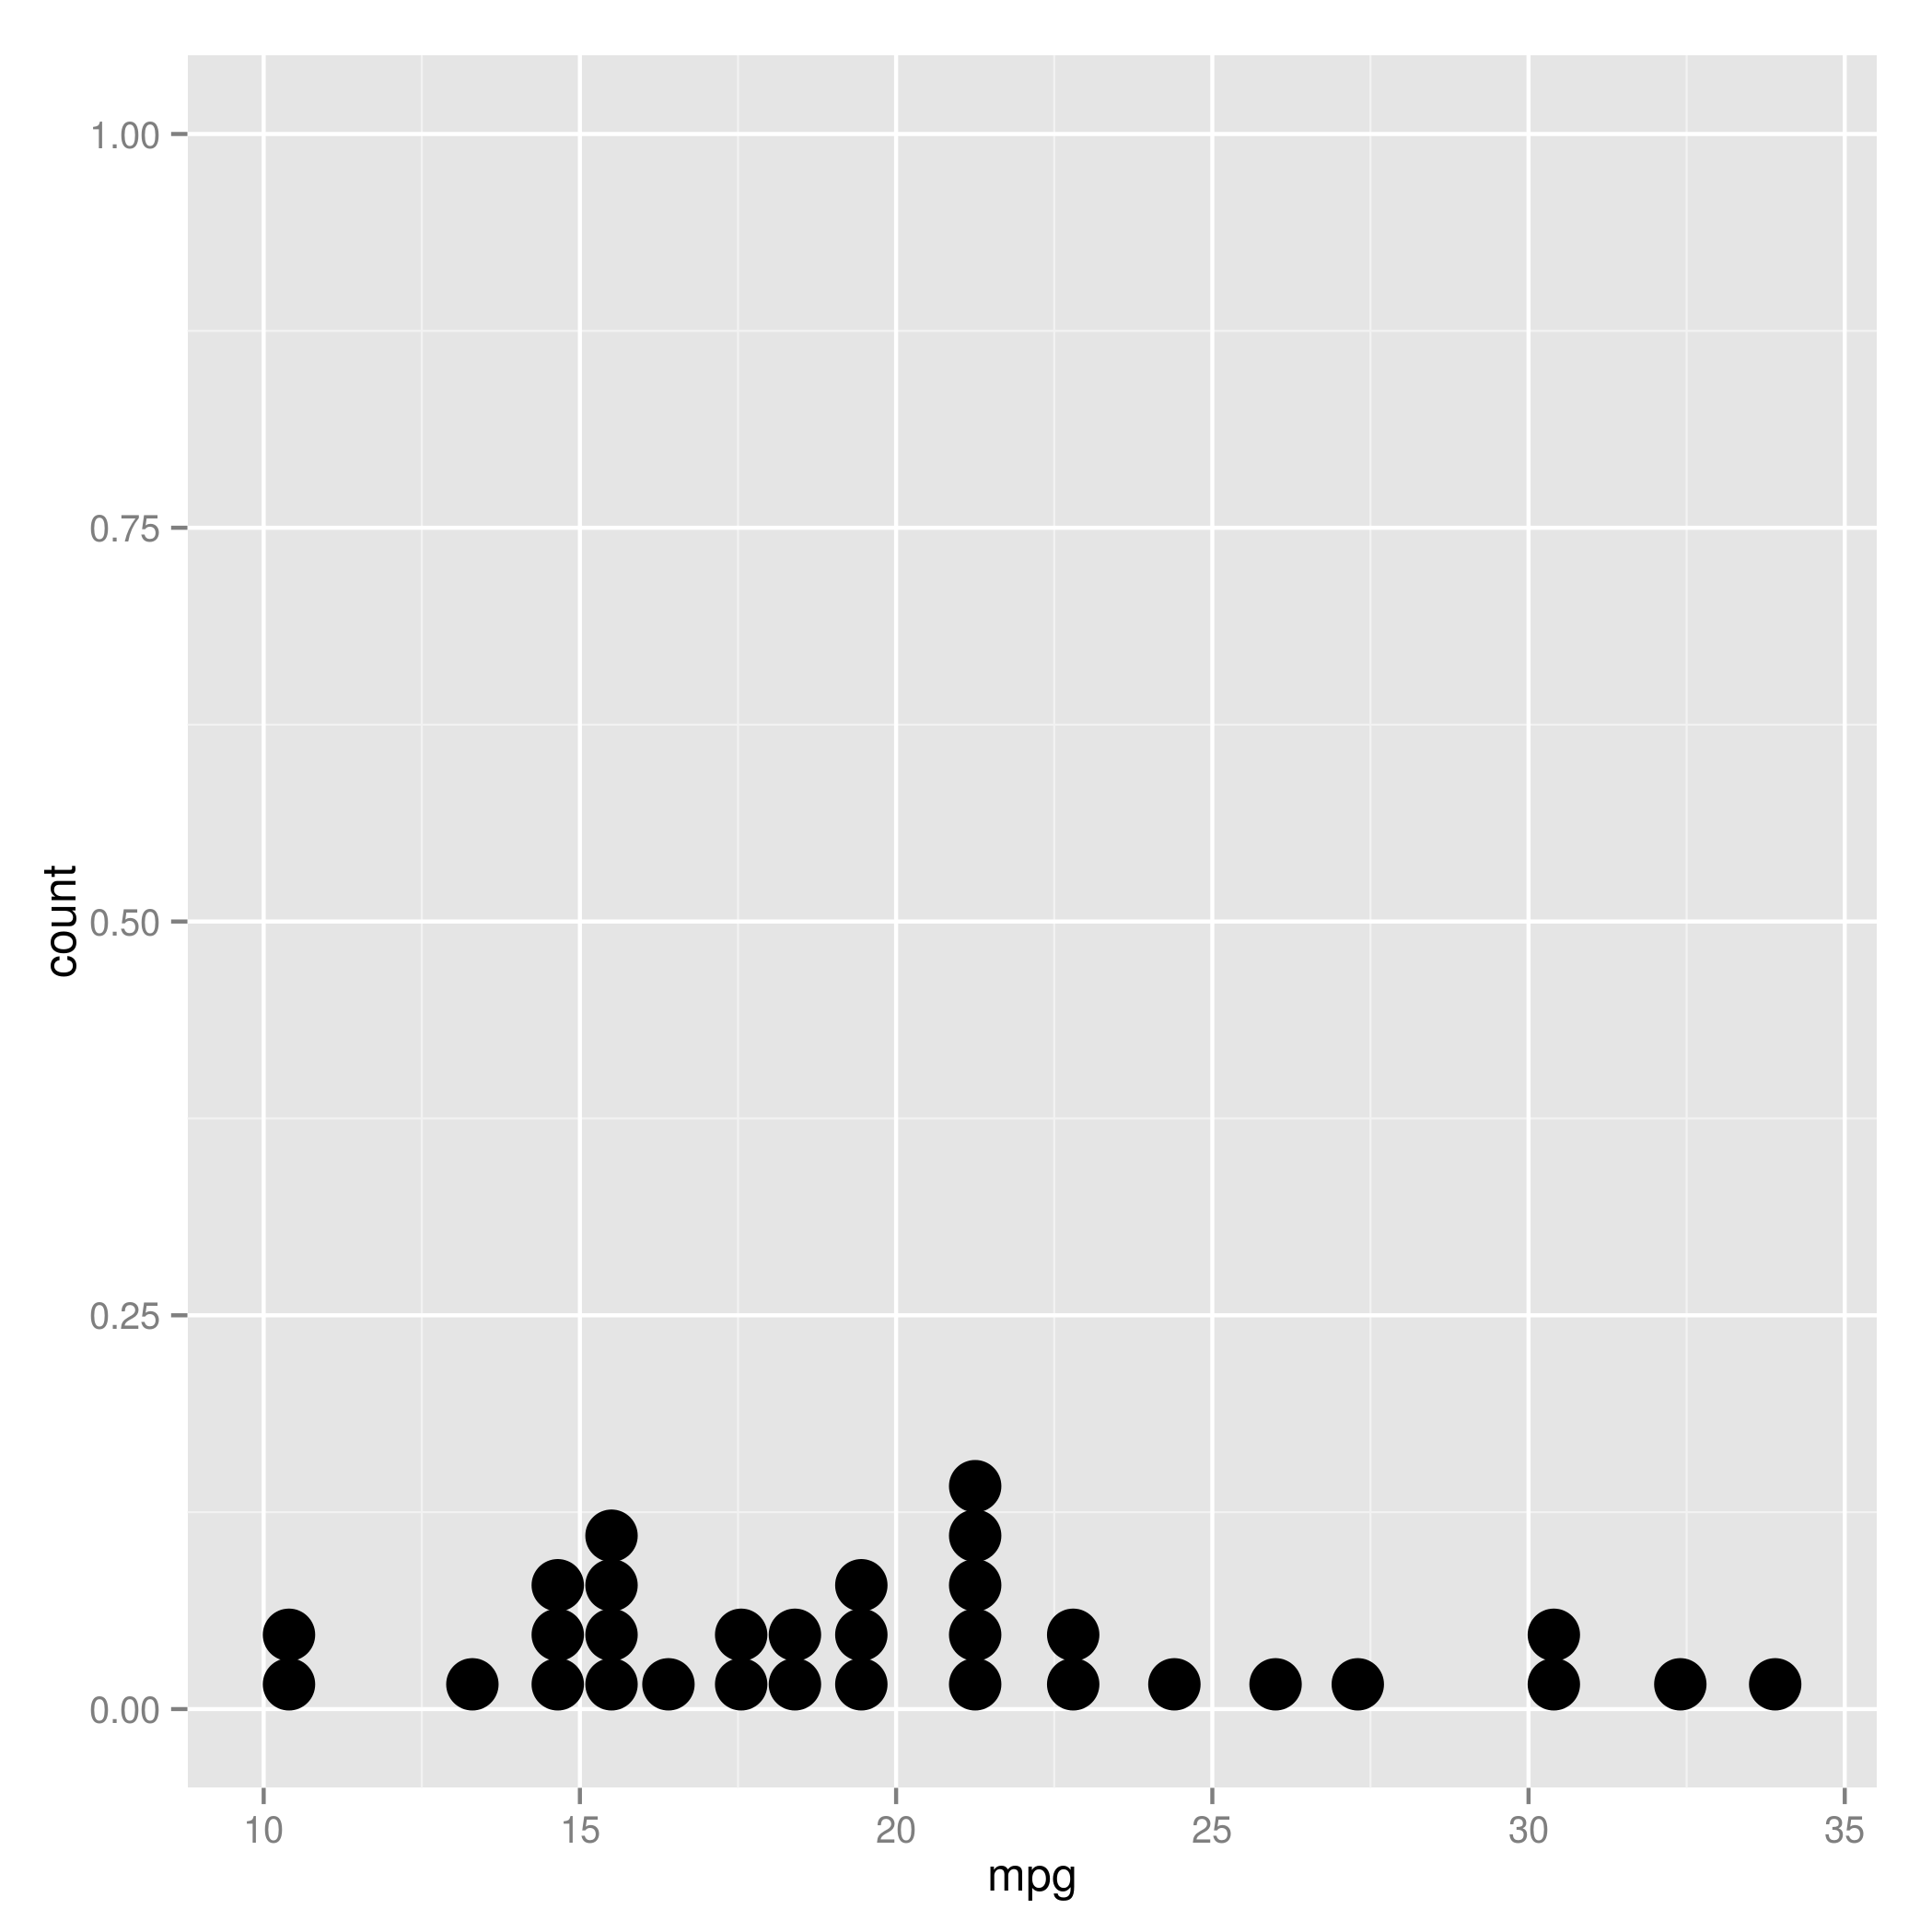
\includegraphics[width=8cm]{dotplot1.png}
  \end{center}
\end{frame}



\begin{frame}[fragile]\frametitle{geom\_dotplot()}
\small
\begin{verbatim}
> ggplot(mtcars, aes(x = mpg)) + geom_dotplot(binwidth = 1.5)
\end{verbatim}
which results in:
\end{frame}

\begin{frame}\frametitle{dot plot example}
  \begin{center}
    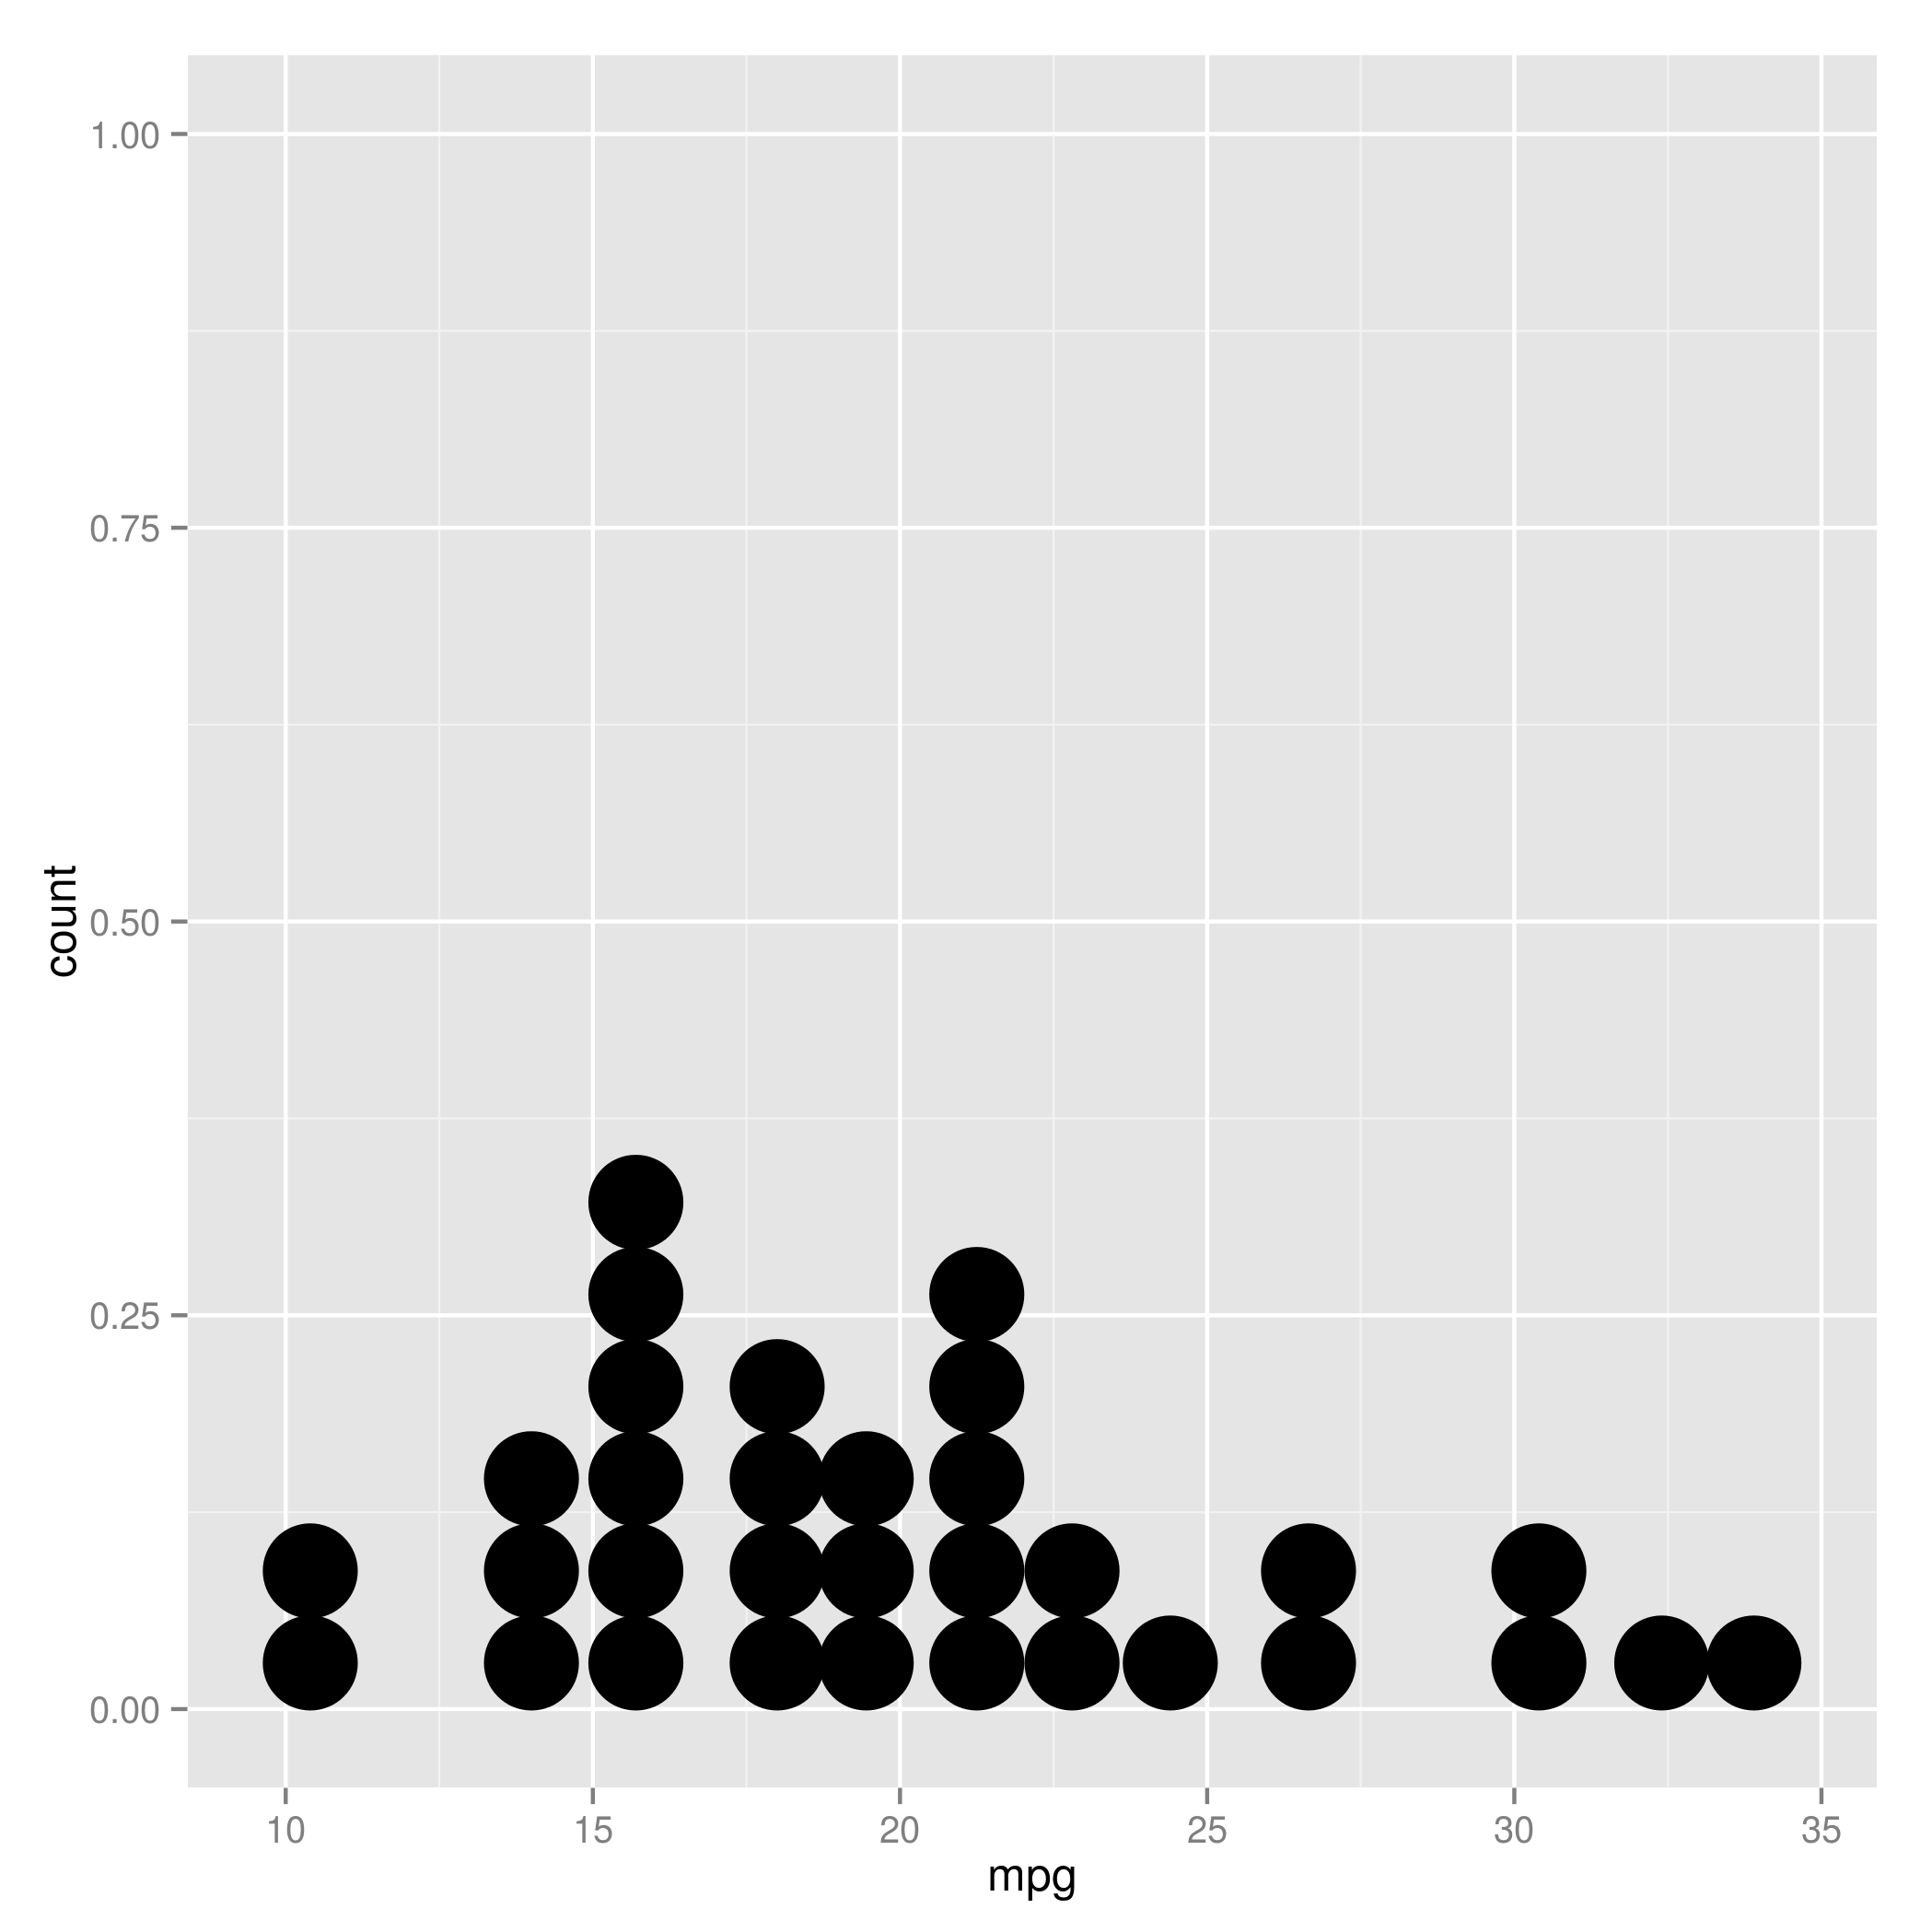
\includegraphics[width=8cm]{dotplot2.png}
  \end{center}
\end{frame}



\begin{frame}[fragile]\frametitle{geom\_dotplot()}
\small
\begin{verbatim}
> ggplot(mtcars, aes(x = mpg)) +
+     geom_dotplot(binwidth = 1.5, stackdir = "center")
\end{verbatim}
which results in:
\end{frame}

\begin{frame}\frametitle{dot plot example}
  \begin{center}
    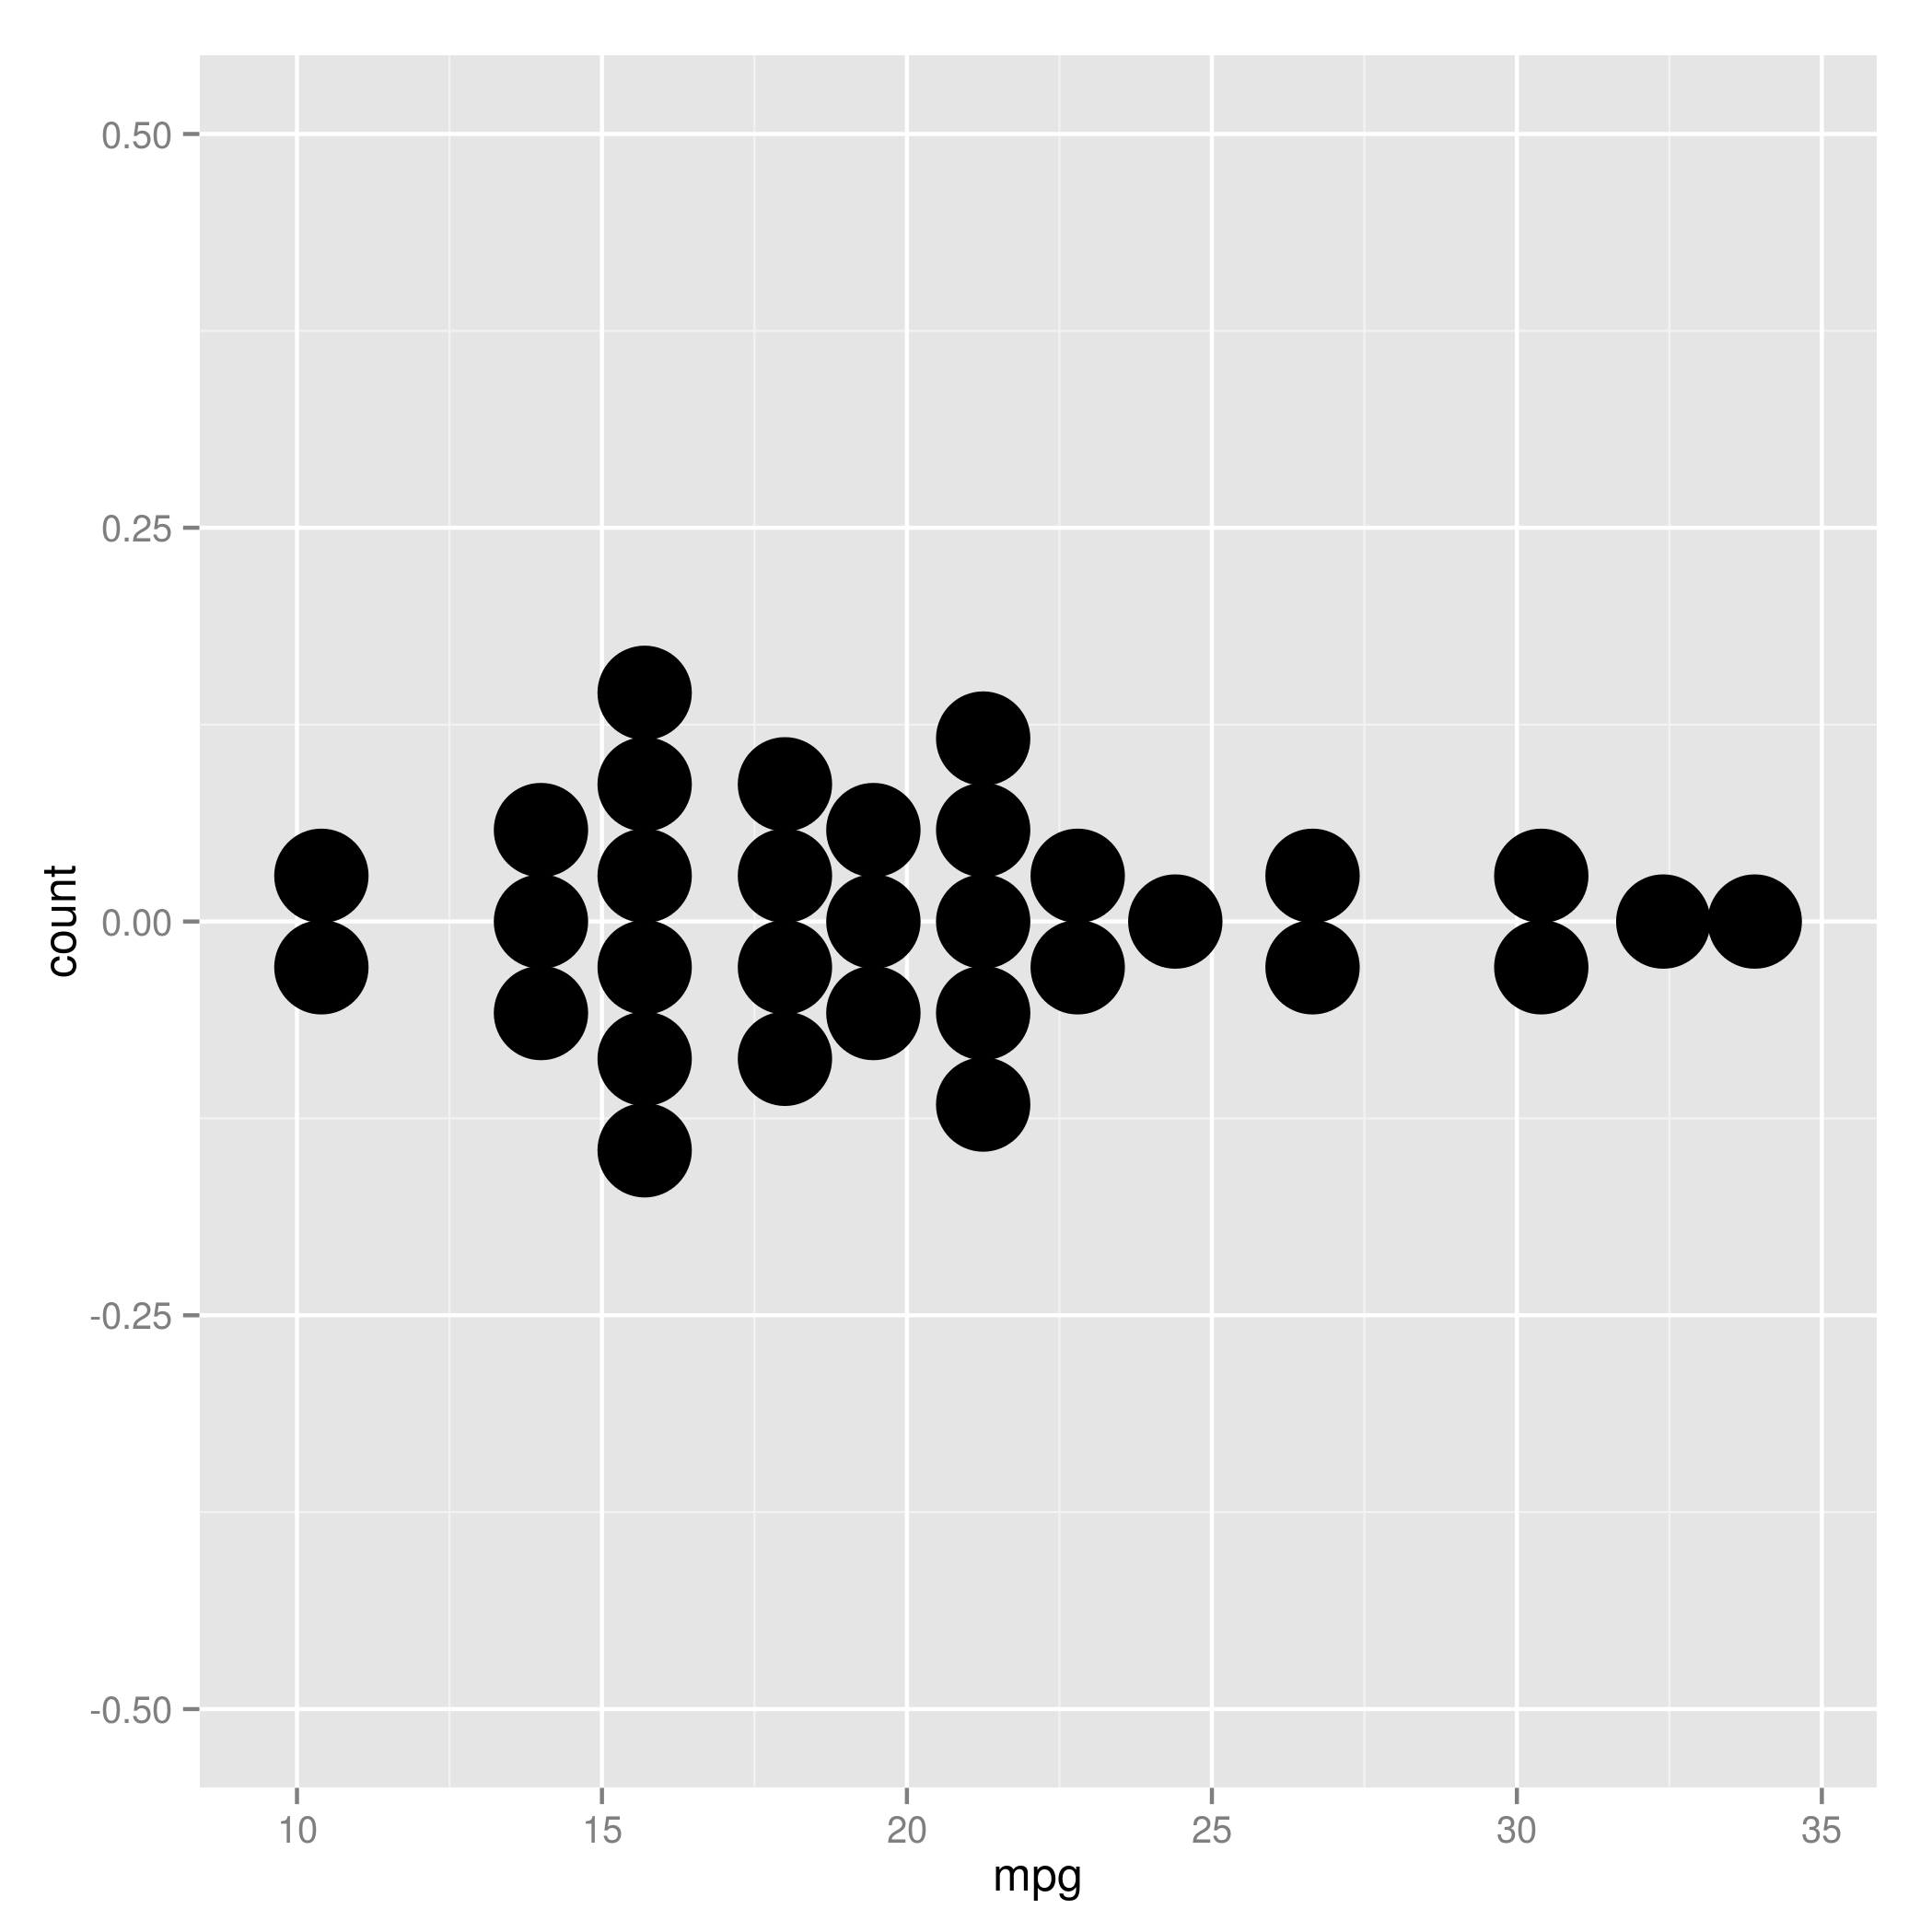
\includegraphics[width=8cm]{dotplot4.png}
  \end{center}
\end{frame}




\begin{frame}[allowframebreaks]\frametitle{Exercises}
  \begin{enumerate}
  \item use again the GaltonFamilies data set; produce a scatter plot of \texttt{childHeight} vs \texttt{midparentHeight}
  \item add a trend line by using \texttt{geom\_smooth()} without any arguments. Which method is used?
  \item add a second trend line, this time a linear one!
  \item now map the aesthetic \texttt{colour} to \texttt{gender} in the first line of the plot definition. What happens?
  \end{enumerate}
\end{frame}

\section{Some News}
\subsection{from useR2015}

\begin{frame}\frametitle{INBOthemes}
  \begin{itemize}
  \item provides ggplot theme for elsevier and some nice color palettes
  \item new in Rstudio 0.99
    \begin{itemize}
    \item data viewer displays more than 1000 lines
    \item provides now filter and sort function
    \item better completion
    \item code diagnostics etc...
    \end{itemize}
  \item density legends (OpenAnalytics) 
  \end{itemize}

\end{frame}

\section{Last Session}

\begin{frame}\frametitle{What we've learned}
  \begin{itemize}
  \item there are different tests of location, in general we can distinct 
    \begin{itemize}
    \item parametric and
    \item non-parametric tests
    \end{itemize}
  \end{itemize}
\end{frame}

\begin{frame}\frametitle{What we've learned}
  \begin{itemize}
  \item parametric test(s):
    \begin{itemize}
    \item t-tests
    \end{itemize}
  \item non-parametric test(s):
    \begin{itemize}
    \item Wilcoxon tests
    \end{itemize}
  \end{itemize}
\end{frame}

\begin{frame}\frametitle{What we've learned}
  \begin{itemize}
  \item if we talk about testing you should know the definition of the following terms, (a)  for a one sample (b) for a two sample t-test 
    \begin{itemize}
    \item Null hypothesis
    \item Alternative hypothesis
    \item Test statistic
    \item Significance level
    \item Critical value
    \item Decision rule
    \item Type I error
    \item Type II error
    \item (Power)
    \end{itemize}
  \end{itemize}
\end{frame}

\begin{frame}[fragile]\frametitle{Exercise}
Lloyd et al (1969) studied the transferal of tritiated water (water containing a radioactive isotope of hydrogen with detrimental health effects) across the human chloroamnion (placental membrane). Permeability to tritium was measured for two groups of membranes, A and B. The data are\small
\begin{verbatim}
> data <- data.frame(values = c(0.8,0.83,1.89,1.04,1.45,
                                1.38,1.91,1.64,0.73,1.46,
                                1.15,0.88,0.9,0.74,1.21),
                     membrane = rep(LETTERS[1:2],c(10,5)))
\end{verbatim}\normalsize
\begin{enumerate}
  \item check normality using histograms (and/or normal probability plots - \texttt{geom\_qqplot()})
  \item Conduct a Wilcoxon rank sum test (\texttt{wilcox.test()}) for the alternative hypothesis that A is greater than B.
  \end{enumerate}
\end{frame}


\begin{frame}[fragile]\frametitle{Exercise}
To compare two different weight loss programs ($X$ and $Y$) and to control of the confounding potential of genetics, 12 pairs of identical twins of similar weight were studied. Each paire of twins was randomly assigned to program $X$ or $Y$ and the amount of lost weight in pounds was recorded. Test if program $X$ is superior to program $Y$.
  \begin{enumerate}
  \item State your hypothesis.
  \item Do the appropriate test.
  \item visualize.
  \item State your conclusion.
  \end{enumerate}
\textit{Hint:} The \texttt{granovaGG} package contains a function \texttt{granovagg.ds()} to visualize dependent samples. Try this plot and try to understand the plot elements.
\end{frame}


\begin{frame}[fragile]\frametitle{Exercise}
  \begin{enumerate}
  \item Install the \texttt{asbio} package and load the data set magnets using the \texttt{data()} command.
  \item by typing the question mark followed by the name of the data set you get a description of the data
\begin{verbatim}
> ?magnets  
\end{verbatim}
\item read this description. The question was \textit{Was the pain reduction in the magnet group superior}. We assume a t-test is appropriate. Do all necessary steps to answer this question.
  \end{enumerate}
\end{frame}

\end{document}
